
%Corps du document :
%\setlength{\parindent}{1cm}    

\section{Introduction}

Le but de ce dossier d'initialisation est de poser les bases nécessaires au bon déroulement du projet d'ingénierie. Nous répondons dans l'ensemble des documents produits par l'hexanôme H4111 à l'appel d'offre lancé par le COPEVUE visant à concevoir un Système de monitoring à distance de sites isolés. Dans ce document sont détaillés les constituants même du projet. Nous insisterons donc sur les points de vue organisationnels liés à la conception de notre solution technique.Après avoir resitué le contexte du problème, il s'agira de définir les objectifs ainsi que les contraintes liés à ce type de projet. Sont détaillées aussi dans ce document, les méthodes de travail,la répartition des rôles au sein du groupe d'ingénierie ainsi que le planning de répartition des tâches et des charges de travail. Une description précise des livrables sera effectuée et nous donnerons un aperçu des risques que nous sommes susceptible de rencontrer.

\section{Contexte du document}
Dans le cadre d'un projet d'ingénierie, l'utilité d'un dossier d'initialisation est double. Tout d'abord, celui-ci permet de préciser au client quelle seront les modalités formelles des documents et des livrables qui lui seront fournis. Ce dossier permet de lancer le projet en ce qu'il pose les bases et détaille le contenu de ce que le groupe d'ingénierie va produire tout au long des phases de vie d'un projet (spécification, conception, réalisation, tests, intégration, recette…).D'autre part, ce dossier d'initialisation sert de référentiel commun au groupe de travail. Il permet de clarifier les procédures de travail au sein du groupe humain. Ainsi s'il arrive qu'un acteur s'éloigne de ses objectifs principaux, il suffira de se référer au dossier d'initialisation pour recadrer son travail. Le Macro-Phasage permet de même de prévoir l'évolution du travail et de constater les éventuels écarts de entre ce qui avait été prévu et ce qui a été réellement fait, c'est donc un outil de gestion de risque.
\section{Documents de référence}
%que mettre dans cette partie->voir avec Jan.
    
\section{Rappel du problème}
Le COPEVUE a lancé un appel d'offre dans le cadre de la réalisation d'un système de monitoring de sites isolés. Il s'agit donc de concevoir en premier lieu une solution technique permettant de répondre aux mieux aux exigences fonctionnelles et non fonctionnelles que le COPEVUE formule. De façon synthétique notre équipe va proposer une solution permettant de surveiller des sites naturels difficiles d'accès (souvent à cause des conditions environnementales) et peu peuplés. Dans ces sites isolés sont souvent regroupés des postes de travail et ces zones doivent pouvoir être surveillées en dépit de la distance qui les sépare du bureau de contröle.
\subsection{Le contexte}
Notre cas d'étude se limite pour l'instant à considérer une situation simple : comment pouvoir maintenir de manière rentable des réserves de tel ou tel composé à un niveau correct bien que le site de stockage soit situer dans des zones difficiles d'accès ? L'idéal serait donc de pouvoir suivre a distance l'évolution d'un niveau d'un composé en fonction du temps.Le ravitaillement serait ainsi plus raisonnable car on saurait alors la quantité de composant à acheminer sur place. Trouver une solution fonctionnelle à cette problématique permettrait ainsi d'économiser en frais de maintenance mais aussi et surtout d'éviter certaines catastrophe écologique comme par exemple un manque d'eau dans un réservoir lors d'un feu de forêt ou encore une fuite de carburant d'un réservoir de forêt.

\subsection{Les objectifs}
Il s'agit donc d'étudier et de concevoir un système autonome et qui pourra être adapté à de nombreux sites autour du monde (autant dans les zones chaudes que dans les zones froides) de mesure et de monitoring à distance de zones de travail isolées. Il devra être possible de même d'éffectuer des actions de pilotage, de configuration et de maintenance des zones. Il est intéressant de rester assez général dans les différentes actions qu'il sera possible de mener à distance afin d'avoir une solution évolutive qui saura s'adapter à d'autres cas de figure.
Voici quelques éléments permettant d'esquisser un système qui pourrait convenir :

\begin{itemize}
\item Choisir une batterie de capteurs adpatés aux différents sites à couvrir.
\item Concevoir l'architecture d'un système collectant les données.
\item Stocker les données récupérées dans toutes les zones sur un serveur distant.
\item Traiter ces données pour les restituer à un utilisateur.
\item Permettre d'agir sur le système par des fonctions simples (ordre de ravitaillement, de nettoyage …)
\item Pouvoir faire évoluer le système vers des surveillances de zones plus complexes.
\end{itemize}
    
\section{Les contraintes générales}
Dans ce projet, il sera important de bien calculer les surcoûts éventuels liés au développement du système. Nous veillerons à garde notre solution compétitive vis à vis des autres solutions disponibles sur le marché. Il faudra de même prendre en compte le coût de maintenance et d'exploitation d'un tel système.

\subsection{Etude de l'existant}
\subsubsection{Solution existante interne à COPEVUE}
Il n’existe actuellement aucun système de monitoring de site isolés en sein du COPEVUE. A ce jour, les sites isolés sont non automatisés, ils sont surveillés manuellement. Il n’existe aucune communication entre les sites et un quelconque serveur, ce qui necessite un déplacement constant pour maintenir les installations. Ce déplacement entraine un coup important.Il n’existe actuellement aucune entreprise ou projet qui permet de répondre à notre cahier des charges. Cependant, certains d’entre eux ce rapproche suffisament de notre cas, nous allons lister ici les informations utiles à leur sujet.
	\subsubsection{Solution existante concurrente}
\begin{itemize}
\item One Touch Automation :
C’est l’entreprise qui se rapproche le plus de notre futur système. Cette entreprise permet un système de monitoring abouti grâce à une très basse consommation de leurs outils. Ils surveillent des sites isolés grâce à des caméras de surveillance CCTV alimentés par un système hybride solaire/éolien. Le système est portable ou fixe.
\item MeerCam :
Système de surveillance automatisé de bâtiment grâce à des caméras basse consommation. Ces caméras sont équipés de trois batteries permettant une durée de vie de quatre ans.
\item boitier ElOcom :
Les boitiers ELOcom équipent un réseau de camion. Ce système permet la localisation et la télécommunication avec un serveur distant (liaison CANbus entre l’antenne GSM et le GPS).
\end{itemize}

    \subsection{Exigences fonctionnelles}
\begin{itemize}
\item Le système doit pouvoir récupérer des données de capteurs tout autours du monde.
\item Les informations récoltées par le sytème doivent être accessible à l'aide de plusieurs plateformes.
\item Comme pour le point précédent les commandes doivent pouvoir être transmises depuis plusieurs plateforme.
\item Le système doit être très peu grourmand en énergie car celle-ci sera parfois rare dans les régions à équiper.
\item Le système doit être complètement autonome car l'intervention humaine sur ce type de zone est rare.
\item Le point précédent impose que l'on puisse maintenir et configurer le système à distance.
\item Le système doit supporter des conditions environementales très rude (de -50 degrès à 50 degrès environ).
\item Le système doit pouvoir signaler un problème technique au sein même de son fonctionnement.
\end{itemize}

    \subsection{Exigences non fonctionnelles}
\begin{itemize}
\item INTEGRATION DE L EXISTANT : réaliser un système en adéquation avec les personnes qui travaillent déjà à la surveillance des sites sensibles, à savoir les camionneurs.
\item ROBUSTESSE : le système doit toujours redémarré dans un état stable suite à des éventuels pannes ou redémarrage.
\item FIABILITE : le système ne doit pas bugger ou se bloquer car tout réparage sur site du sytème est à proscrire.
\item EVOLUTIVITE : le système conçu à l'origine pour la surveillance de cuves doit pouvoir s'adapter à de nouvelles conditions environnementales.
\item TECHNOLOGIES : le système devra utiliser les technologies GPS et GPRS.
\item GENERICITE : le système doit pouvoir être adapté rapidement à de nouvelles situations, il serait intéressant de considérer une démarche de progicialisation.
\item REUTILISATION : le système conçu doit se reposer sur des technologies logicielles connues et aisément réutilisables. Il sera nécessaire de préciser quels seront les composants réutilisable.
\item ERGONOMIE : Afin de transmettre l'information rapidement à un non informaticien, il faudra adapter l'IHM à la plateforme de travail et veiller à ce que les informations soient claires.
\item TRACABILITE : Il est nécessaire de garder un journal d'activité du système, ce journal devra être gardé au minimum 2 ans.
\end{itemize}
   
\section{Organisation du travail}
Le groupe de travail est divisé en 3 entités qui sont :
\begin{itemize}
\item \textbf{Le Chef de Projet} représenté par Mr Alexandre LEFOULON chargé de piloter le projet de réponse à l'appel d'offre lancé par COPEVUE concernant la conception d'un système de monitoring isolé.
\item \textbf{Le Responsable Qualité et Documentation} représenté par Mr Jan KEROMNES chargé de dresser en accord avec les autres membres du projet les règles de travail (gestion des best practices, validation des tâches) à appliquer pour mener à bien la réponse à l'appel d'offres.
\item \textbf{Le Groupe d'Etude Informatique} représenté par Melle Tuuli Tyrvaïnen, Mr Quentin CALVEZ, Mr Matthieu COQUET, Mr Xavier SAUVAGNAT et Mr Thaddee TYL chargés de spécifier et de concevoir une solution technologique en accord avec les besoins du COPEVUE.
\end{itemize}

    
    \subsection{Chef de projet (CdP)}
Le chef de projet sera chargé de la rédaction de certains documents de lancements et organisationnels (ceux-ci sont détaillés plus loin).Il sera de même chargé de répartir le travail au sein de son groupe d'ingénierie. Il doit connaître l'avancement du projet et animer les séances de travail. A l'issue de chacune d'elle il devra dégager un bilan de séance et juger de l'avancement des différentes tâches. Avec l'aide du responsable qualité il veillera à valider chaque document selon les best practices et les modalités de validation définies lors de la phase d'initialisation. Dans le cas ou le projet viendrait à prendre du retard, le chef du projet veillera à redéfinir les axes de travail dont le groupe s'est peut-être trop écarté.Le chef de projet aura de même un rôle fédérateur afin d'emmener le groupe de travail vers la séléction de leur appel d'offre.
    \subsection{Responsable Qualité, Méthode et Documentation}
Le responsable qualité, méthode et documentation sera chargé d'insufler les bonnes pratiques au sein du groupe de travail. Celles-ci permettront ainsi de produire un travail précis et répondant le mieux aux exigences de l'appel d'offre. Ces bonnes pratiques seront symbolisées par des méthodes de travail et par l'utilisation de logiciels et de langage de modélisation précis. Tout comme pour le chef de projet, le RQ sera chargé de la rédaction de certains documents détaillés ci-après. Cet acteur indispensable à la survie d'un projet sera en constante communication avec le GEI afin de veiller à ce que l'application des bonnes pratiques soit effective et n'induise pas un surcoût en temps.
    \subsection{Groupe d'études informatique}
Le groupe d'étude informatique composé de 5 personnes est le noyau dur du groupe de travail. Dans le cadre de la réponse à l'appel d'offre pour la première phase du projet (étude de l'existant, étude de faisabilité et spécification des besoins) les rôles ont été répartis ainsi  :
\begin{itemize}
\item \textbf{Tuuli TYRVAINEN} : est chargée d'étudier les possibilités de production d'énergie dans les pays froids et dont les contraintes d'ensoleillement sont importantes, il s'agit donc des pays proches du cercle polaire (Norvège, Finlande, Suède…).
\item \textbf{Quentin CALVEZ} : est chargé d'étudier les différents moyens de productions et de stockage d'énergie afin de répondre aux contraintes d'économie d'énergie induites par les besoins du COPEVUE. Il sera en lien direct avec Tuuli Tyrvainen afin de gérer le cas des pays nordiques.
\item \textbf{Matthieu COQUET} : est chargé d'éffectuer l'étude de l'existant au sein de COPEVUE ainsi que l'étape de benchmarking visant à prendre des connaissances des éventuelles solutions présentes sur le marché.
\item \textbf{Xavier SAUVAGNAT} : est chargé d'étudier les différents types de capteurs présent sur le marché mais aussi de recenser ceux qui vont pouvoir être utiles dans le cadre de la réalisation de notre système. L'idéal serait de pouvoir chiffrer le coût d'achat de ces capteurs. 
\item \textbf{Thaddee TYL} : est chargé de l'étude de l'OS (ou du RTOS à mettre en place) sur le système d'acquisition des données. Afin d'être en cohérence avec son domaine de compétence, il sera de même chargé d'étudier les différents moyens hardware que notre groupe de travail va utiliser non seulement pour récupérer les données mais aussi pour les transmettre au serveur centrale. 
\end{itemize}

    
    \section{Listes des livrables attendus}
Voici une description des livrables qui seront rendus à l'issue de la phase 1. Ce dossier d'initialisation sera donc recomplété lors du commencement des phases 2 et 3.
    \subsection{Chef de projet}
Livrables du chef de projet :
\begin{itemize}
\item \textbf{Le Dossier d'Initialisation} : Ce document sert de référentiel commun entre le COPEVUE et notre équipe qui proposera une solution. Celui-ci permet de répertorier et de décrire chaque livrable. Pour la plupart des livrables, on définit leurs plan généraux. Ce livrable informera le COPEVUE des étapes d’élaboration de la solution la plus adaptée à la gestion des sites isolés. Le contenu de ce dossier est donc défini selon les parties précisées dans le sommaire (Livrables, Macro-Phasage, Répartition des rôles, Gestion des risques).
\item \textbf{Le Relevé de Décisions} : Dossier rédigé qui rend compte des décisions prisent lors des revues de travail au sein des séances. Il justifiera les décisions concernant en particulier le dossier de faisabilité (pour la phase 1) et sera mis à jour tout au long du déroulement du projet.
\item \textbf{La Fiche d'Argumentation Commerciale} : Ce document permettra de présenter le produit sous un angle commercial. Il donnera une vue synthétique, claire et fonctionnel de notre réponse à l'appel d'offre lancé par le COPEVUE.
\item \textbf{La Rédaction d'une procédure} : Le chef de projet devra rédiger la procédure de son choix à savoir : soit la \og décomposition d'un sytème et choix de sous projets \fg ou \og gestion de configuration \fg.
\item \textbf{Le Plan de Mangement de Projet} : Le PMP doit présenter pour l'ensemble du projet de monitoring de systèmes isolés les livrables et l'organisation fonctionnelle du projet. Ce rapport permet donc de bien délimiter le domaine d'étude de chaque sous-projet.

\end{itemize}

    \subsection{Responsable Qualité}
Livrables du responsable qualité :   
\begin{itemize}
\item \textbf{Le Glossaire Commun} : ce document doit être rempli par tout à chacun au sein du groupe et servira notamment pour la compréhension des termes complexes rencontrés tout au long de la rédaction des dossiers (pour le CdP, le RQ, le GEI).
\item \textbf{Le Dossier de structuration de la documentation et d'organisation de la production} : Dossier précisant les processus à appliquer pour gérer la production et la gestion des documents à fournir au client. Ce document a l'avantage qu'il s'agit d'un point d'attache procédurale et que chacun peut aller se renseigner dedans sur les règles impératives à appliquer lorsque l'on rédige un document.
\item \textbf{La Rédaction de la Best Practice 1} : cette Best Practice devra répondre à la problématique \og Comment rédiger une bonne procédure ?\fg. Ce dossier rédigé permet d'amorcer le travail de rédaction de procédure du chef de projet. Ce document est détaché du domaine technique de notre étude mais permet cependant de poser les bases et de donner les consignes nécessaires à la rédaction d'une procédure. Le RQ devra définir les éléments clefs en insistant sur le domaine pratique de ce type de document.
\item \textbf{Rédaction du dossier de synthèse} : ce document permet au RQ de se faire une idée générale des choix techniques pris par l'équipe GEI et le chef de projet. Ce dossier présente donc une synthèse des améliorations que notre groupe de travail va apporter au système déjà existant, c'est donc l'essentiel du projet qui est présenté ici. Ce dossier permettra au COPEVUE d'avoir l'éssentiel de notre travail en un document clair et concis.
\item \textbf{PAQP} :  Ce document doit définir l’ensemble des règles pour garantir l’intégration et la réussite du projet.
\end{itemize}

    \subsection{Groupe d'études informatique}
Livrables du Groupe d'études informatique:   
\begin{itemize}
\item \textbf{Dossier de faisabilité} : Ce dossier permet de prendre connaissance des possibilités qui s'offrent à nous dans les domaines techniques qui nous touchent pour la réponse à l'appel d'offre. Le GEI va donc étudier les différentes sortes de capteurs aujourd'hui présent sur le marché mais aussi tout ce qui sera autour, à savoir ce qui va nous permettre de transmettre l'information, ou encore de la stocker. D'une manière encore sommaire, le groupe GEI se fera une idée dont seront agencés les appareils que nous choisissont.
\item \textbf{Le Dossier de spécification technique des besoins} : Ce dossier récapitule les besoins techniques transmis par le biais de l'appel d'offre. Ces besoins seront donc traduits en exigences fonctionnelles et non fontionnelles. Enfin, notre groupe de travail définira les axes de progrès à apporter au projet.
\item \textbf{Le Dossier de conception détaillée du système} :  C'est l'initialisation de la partie conceptuelle du projet. Nous nous attacherons à préciser l'architecture générale du système et à commenter l'assemblage plus précis des différents composants qui entrent en jeu.
\item \textbf{Les cahier des charges logiciels} :  Ce sont les cahiers des charges qui définissent les exigences des éléments logiciels qu'il sera nécessaire de développer dans le cadre de tel ou tel sous-projet. Pour avoir plus d'informations sur le contenu de ces sous-projet, voir le PMP.

En plus de ces livrables client, chaque ressource sera chargée de rédiger un bilan personnel rendant compte de son expérience au sein du groupe de travail H4111.

\end{itemize}

\section{Taches du projet de réponse à l'appel d'offre}
\subsection{Phase 1}
séance 1 
\begin {center}
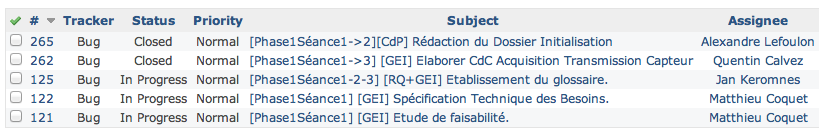
\includegraphics[width=\textwidth]{png/Phase1Seance1.png}
\end {center}
séance 2
\begin {center}
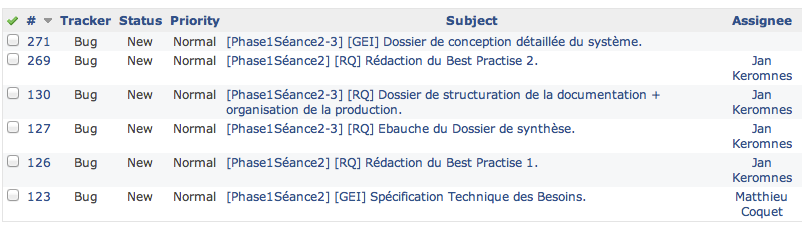
\includegraphics[width=\textwidth]{png/Phase1Seance2.png}
\end {center}
séance 3
\begin {center}
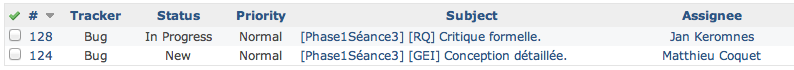
\includegraphics[width=\textwidth]{png/Phase1Seance3.png}
\end {center}
\subsection{Phase 2}
séance 1
\begin {center}
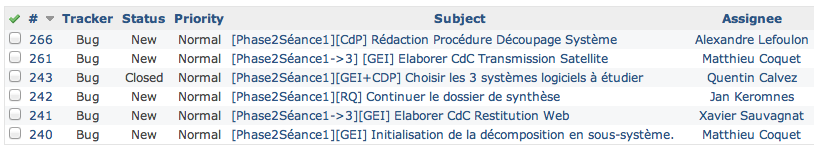
\includegraphics[width=\textwidth]{png/Phase2Seance1.png}
\end {center}
séance 2
\begin {center}
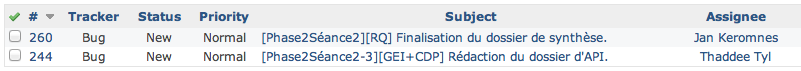
\includegraphics[width=\textwidth]{png/Phase2Seance2.png}
\end {center}
séance 3
\begin {center}
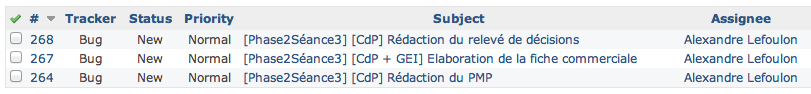
\includegraphics[width=\textwidth]{png/Phase2Seance3.png}
\end {center}

\subsection{Diagramme de Gantt}
Voici le diagramme de gantt du projet de réponse à l'appel d'offre. 
\begin {center}
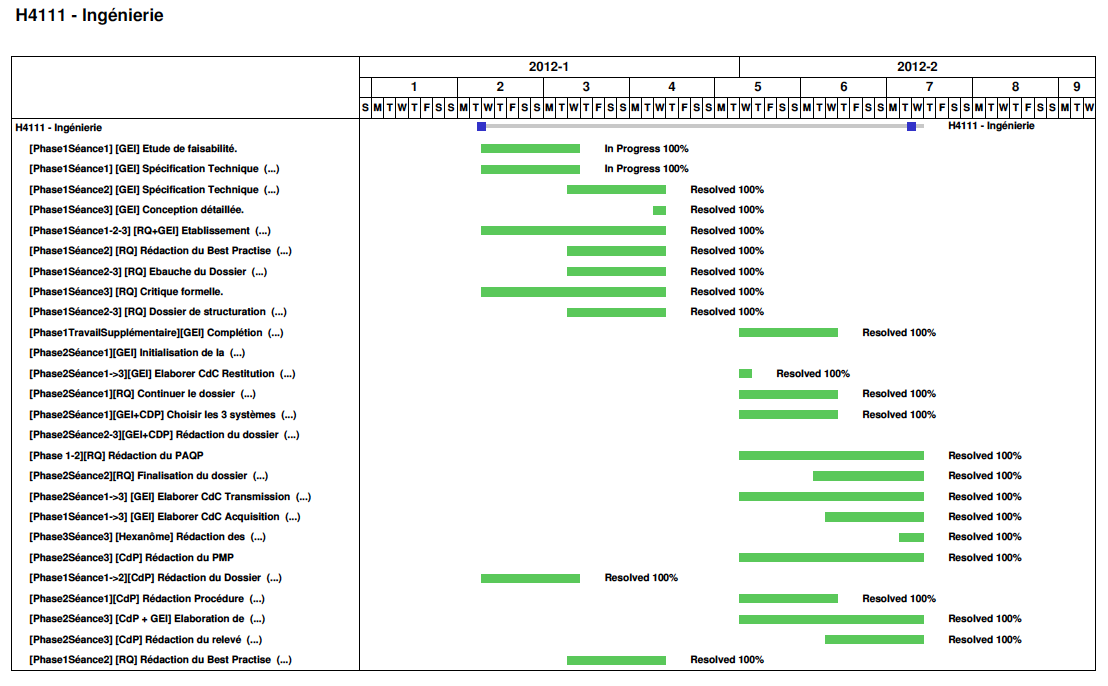
\includegraphics[width=\textwidth]{png/Gantt.png}
\end {center}

    
    \section{Modalités de validation}
Nous détaillerons dans cette partie quelles sont les étapes à respecter pour réaliser un document. Dans tous les cas, si un membre rencontre un problème inattendu, il devra l’informer au chef de projet. Celui-ci pourra en prendre compte pour mieux organiser ces tâches dans le futur.
     \subsection{Les règles de suivi}
Réalisation et validation par le groupe chargé de la tâche :
Si plusieurs personnes sont chargées d’une même tâche, la réalisation de la tâche se fera en présence de tout les membres du groupe. Une fois que la réalisation semble terminé, les membres doivent impérativement auto valider leur travail. Ils effectuerons une relecture du documents et vérifierons que tous les objectifs ont été atteints. Pour terminer, chaque personne doit compléter la quantité de temps passée sur la tâche.

Validation par le responsable qualité :
Une fois le document rédigé et valider par le groupe. Le responsable qualité s’assure que la réalisation est conforme au PAQ. Si un ou plusieurs points semblent incorrectes, la tâche est repassé en étape de réalisation par les mêmes membres.

Validation par le chef de projet:
Le chef de projet validera une fois que le responsable qualité aura accepté le documents. Une fois ceci fait, la tâche est valider et le document ne doit plus être modifié, sauf si cela rentre dans une nouvelle tâche demandé par le chef de projet.

    \subsection{Les outils utilisés}
Listes des différents outils et méthodes qui seront utilisés tout au long du projet:
\begin{itemize}
\item \textbf{Google Docs} : Outil en ligne permettant un partage et un travail simultané en temps réel sur différents types de documents, avec une gestion des versions. Ne sera utilisé que le temps de la mise en place d’outils plus avancés.
\item \textbf{UML} : langage de modélisation, qui sera surtout utilisé pour la modélisation des cas d’utilisation.
\item \textbf{Redmine} : Gestionnaire de projet en ligne, disposant d’un wiki, permettant de suivre le temps passé sur une tâche, d’attribuer les tâches aux différents utilisateurs, de créer un  diagramme de Gantt pour faciliter le travail du chef de projet.
\item \textbf{Git} : Gestionnaire de sources, qui sera intégré directement à Redmine, permettant de travailler à plusieurs sur un même document et de résoudre facilement les conflits au moment de la mise en commun.
\item \textbf{LaTeX} : Langage et système de composition de documents, qui a l’avantage d’être textuel, et donc plus facile à versionner que des documents binaires Office.
\item \textbf{Diagramme de Gantt } : Outil permettant l’ordonnancement et la visualisation des tâches entre les différents membres du projet, afin de gérer au mieux l’avancement du projet.
\end{itemize}

    \subsection{Procédures de révisions du planning}
Ce dossier d'initialisation ainsi que le planning d'activité sera susceptible d'être modifié à l'initialisation de chaque phase du projet.    
    \section{Gestion des risques}
Nous avons relevé la liste des risques perçus :
\begin{itemize}
\item Des risques financiers : qui seront matérialisés dans notre cas par des risques de surcharges de travail. Si l’on passe trop de temps à produire des solutions pour ce projet, nous allons perdre en rentabilité de travail et l’investissement en temps de chacun ne sera pas récompensé à sa juste valeur.
\item Des risques humains : Si une ressource tombe malade, le projet prendra indéniablement du retard et pourra avoir des retards de livraisons. Il arrive aussi parfois qu’une ambiance de stress s’installe au sein du groupe de travail. Ceci peut parfois se produire lorsqu’une revue de travail s’est mal passée ou que le client n’est pas satisfait de la réception de tel ou tel livrable.
\item Des risques organisationnels : Si le temps prévu pour le projet est mal quantifié, le projet ne suivra pas ses lignes directrices et on aura un décalage entre ce qui se passe réellement et ce qui avait été prévu. Ceci entraine donc souvent des retards de livraisons et a un impact importants sur les ressources humaines puisque celles-ci sont alors parfois contraintes de travailler sous la pression.
\end{itemize}

    \subsection{Plans d'actions pour gérer ces risques}
Palier aux risques financiers : Bien chiffrer le projet qui va être réaliser, pour cela, celui-ci doit être parfaitement segmenté. Il est nécessaire d’anticiper et de prévoir les causes des dépenses imprévues. Une possibilité est donc de prendre un intervalle de sécurité en terme de finances (et donc en termes de temps dans notre cas). 

Palier aux risques humains : Le fait que des ressources tombent malade est prévisible au sein du projet, ces retards temporels doivent être pris en compte dans l’intervalle de sécurité établi lors du chiffrage du projet. L’établissement d’une ambiance de stress peut être gérée en recadrant l’équipe de travail et en identifiant les causes du retard. Lorsque l’on connaît les causes il est plus facile de supprimer les mauvaises pratiques et ainsi de remettre le projet dans la bonne direction. Plus les mauvaises pratiques sont décelées vite moins le projet s’écartera du planning prévisionnel.   

    
    \section{Conclusion}
Ce dossier est le point de départ à la réponse que nous allons fournir durant le cycle de travail, il est important de voir que celui-ci doit constituer un référentiel commun à tous les groupes de travail. Il sera important de savoir jongler en termes de temps entre ce projet d'ingénierie et le pld-spie très consommateur en temps lui aussi. Ce dossier a été élaboré durant toute la continuité du projet.   
